\documentclass[11pt]{article}
\usepackage{amstex}
\usepackage[dvips]{epsfig}

\begin{document}
  
\begin{center}
{\LARGE\bfseries{Appendix to Lecture 4: 
Remarks on renormalization and asymptotic freedom} }\\
\vskip 1em%
{\Large Edward Witten}\footnote{\tt 
Notes by Pavel Etingof and David Kazhdan} 
      \vskip 1.5em%
    {\large December 1996} \\ 
\end{center}


\def\top{{\text{top}}}
\def\Re{\text{Re}}
\def\tW{\tilde W}
\def\Aut{\text{Aut}}
\def\tr{{\text{tr}}}
\def\ell{{\text{ell}}}
\def\Ad{\text{Ad}}
\def\u{\bold u}
\def\m{\frak m}
\def\O{{\cal O}}
\def\tA{\tilde A}
\def\qdet{\text{qdet}}
\def\k{\kappa}
\def\RR{\Bbb R}
\def\be{\bold e}
\def\bR{\overline{R}}
\def\tR{\tilde{\cal R}}
\def\hY{\hat Y}
\def\tDY{\widetilde{DY}(\g)}
\def\R{\Bbb R}
\def\h1{\hat{\bold 1}}
\def\hV{\hat V}
\def\deg{\text{deg}}
\def\hz{\hat \z}
\def\hV{\hat V}
\def\Uz{U_h(\g_\z)}
\def\Uzi{U_h(\g_{\z,\infty})}
\def\Uhz{U_h(\g_{\hz_i})}
\def\Uhzi{U_h(\g_{\hz_i,\infty})}
\def\tUz{U_h(\tg_\z)}
\def\tUzi{U_h(\tg_{\z,\infty})}
\def\tUhz{U_h(\tg_{\hz_i})}
\def\tUhzi{U_h(\tg_{\hz_i,\infty})}
\def\hUz{U_h(\hg_\z)}
\def\hUzi{U_h(\hg_{\z,\infty})}
\def\Uoz{U_h(\g^0_\z)}
\def\Uozi{U_h(\g^0_{\z,\infty})}
\def\Uohz{U_h(\g^0_{\hz_i})}
\def\Uohzi{U_h(\g^0_{\hz_i,\infty})}
\def\tUoz{U_h(\tg^0_\z)}
\def\tUozi{U_h(\tg^0_{\z,\infty})}
\def\tUohz{U_h(\tg^0_{\hz_i})}
\def\tUohzi{U_h(\tg^0_{\hz_i,\infty})}
\def\hUoz{U_h(\hg^0_\z)}
\def\hUozi{U_h(\hg^0_{\z,\infty})}
\def\hg{\hat\g}
\def\tg{\tilde\g}
\def\Ind{\text{Ind}}
\def\pF{F^{\prime}}
\def\hR{\hat R}
\def\tF{\tilde F}
\def\tg{\tilde \g}
\def\tG{\tilde G}
\def\hF{\hat F}
\def\bg{\overline{\g}}
\def\bG{\overline{G}}
\def\Spec{\text{Spec}}
\def\tlo{\hat\otimes}
\def\hgr{\hat Gr}
\def\tio{\tilde\otimes}
\def\ho{\hat\otimes}
\def\ad{\text{ad}}
\def\Hom{\text{Hom}}
\def\hh{\hat\h}
\def\a{\frak a}
\def\t{\hat t}
\def\Ua{U_q(\tilde\g)}
\def\U2{{\Ua}_2}
\def\g{\frak g}
\def\n{\frak n}
\def\hh{\frak h}
\def\sltwo{\frak s\frak l _2 }
\def\Z{\Bbb Z}
\def\C{\Bbb C}
\def\d{\partial}
\def\i{\text{i}}
\def\ghat{\hat\frak g}
\def\gtwisted{\hat{\frak g}_{\gamma}}
\def\gtilde{\tilde{\frak g}_{\gamma}}
\def\Tr{\text{\rm Tr}}
\def\l{\lambda}
\def\I{I_{\l,\nu,-g}(V)}
\def\z{\bold z}
\def\Id{\text{Id}}
\def\<{\langle}
\def\>{\rangle}
\def\o{\otimes}
\def\e{\varepsilon}
\def\RE{\text{Re}}
\def\Ug{U_q({\frak g})}
\def\Id{\text{Id}}
\def\End{\text{End}}
\def\gg{\tilde\g}
\def\b{\frak b}
\def\S{\cal S}
\def\L{\Lambda}

{\bf 1. Ambiguity in operator products.} 
In the last lecture we considered Lagrangians of the form
$$
{\cal L}=\int d^4x(\frac{1}{2}(\nabla \phi)^2+\frac{m^2}{2}\phi^2+
\frac{g}{4!}\phi^4+\sum_i\e_i(x)\O_i(x)),
$$
where $\O_i$ are local functionals. 
We saw that defining correlation functions of such Lagrangians 
to the first order in $\e_i(x)$ (i.e. $\e_i\e_j=0$) is equivalent
to defining composite operators corresponding to $\O_i$.  
Now let us work to the second order in $\e_i$ ($\e_i\e_j\e_k=0$).
This corresponds to considering products of composite operators. 
Before we considered products of composite operators at non-coinciding 
points $x,y$, and saw that such a product $\O_i(x)\O_j(y)$ is
defined automatically once we have defined $\O_i$ and $\O_j$.
Now we will allow the points $x$ and $y$ to coincide. 
Then, as we know, the product is not automatically defined, and 
its definition requires additional renormalization. 
This means, we have to introduce counterterms in the Lagrangian,
i.e. consider a new Lagrangian of the form 
$$
{\cal L}'={\cal L}+\sum_{i,j,k} 
L_k\e_i(x)R_k\e_j(x)W_k(\L,g)\O_k(x),
$$
where $L_k,R_k$ are differential operators (in $x$) with constant
coefficients, and $W_k$ are some functions which diverge as $\L\to\infty$. 
The functions $W_k$ are usually not uniquely determined and
cannot be chosen canonically. 
 
Let us consider an example. In one of the homework problems 
we computed the 1-loop correction to the 1-particle 
irreducible bosonic 2-point 
function $\Sigma$ in QED. We discussed that this correction 
can be computed (in momentum space) as 
$$
\int e^{ikx}\<J_\mu(x)J_\nu(0)\>dx,\label 1
$$
where $J_\mu(x)=\bar\psi\gamma_\mu\psi$ is the operator of current, and 
the correlator in (1) is in the theory of a free fermion. 
Now, as follows from the above discussion, 
the product $J_\mu(x)J_\nu(x)$ is defined up to operators 
of lower order, and 
the expectation value $\<J_\mu(x)J_\nu(0)\>$ is 
non-uniquely defined, which causes an ambiguity in 
the computation of (1). However, this non-uniqueness occurs
only at $x=0$. In fact, its is easy to show
that the function $\<J_\mu(x)J_\nu(0)\>$ 
is well defined up to adding a multiple of $\delta(x)$.  
Therefore, the ambiguity in (1) is a constant (i.e. is independent of $k$).

In QED, to preserve gauge invariance, it is necessary to choose this 
constant in such a way that the condition $k^\mu\Sigma_{\mu\nu}(k)=0$ 
is satisfied. 
This gives a unique way to fix the constant. 

{\bf 2. Symmetry breaking.}
A symmetry that exists in a classical field theory may be lost in 
a particular renormalization
scheme for the corresponding quantum theory.
Of course it is possible that there exists a better scheme
which preserves this symmetry, but it is also possible 
that there exists no such scheme, i.e. the symmetry is
broken at the quantum level. For example, consider 
$N$ free massless fermions $\psi_1,...\psi_N$,
with Lagrangian
$\sum (\bar\psi_i,D\psi_i)$, 
$\psi_i\in S_+$, $\Psi_-\in S_-$. In this theory we have 
a $U(N)$ symmetry. Let us add interactions in such a way 
that part of this symmetry is preserved. For example, add a gauge 
field $A$ (i.e. regard the fermions together to make 
a section $\psi$ of the vector bundle $S_+\o E$, 
where $E$ is an $N$-dimensional
Hermitian vector bundle over the spacetime), 
which takes values in the Lie algebra of a subgroup 
$H\subset U(N)$, and consider 
the Lagrangian $(\bar\psi,D_A\psi)$, where $D_A$ is the Dirac 
operator along the connection $A$. 
The classical 
symmetry of this theory is the centralizer $Z(H)$ of $H$. 
In quantum theory, however, this symmetry may fail for topological 
reasons. In other words, a topological anomaly may appear.

{\bf 3. An oversimplified version of experimental confirmation 
of asymptotic freedom.}

Consider a field theory with electromagnetic and strong interactions, 
which contains electrons (which interact only electromagnetically),
and quarks (which interact both electromagnetically and strongly). 
The Lagrangian of such a theory can be written as follows. 
The fields are:


(i) An $SU(3)$-connection $A_g$ (the field of strong interactions),

(ii) A $U(1)$-connection $A_e$ (the electromagnetic field),
 
(iii) Quarks $q_i$ and an electron $\e$ (which are fermions
with values in $\C^3$ and $\C$ respectively).

The Lagrangian is
$$
\int d^4x(\sum_j \bar q_j(iD+A_g+A_e-m_i)q_j+
\bar\e(iD+A_e-m)\e+\frac{1}{e^2}F_{A_e}^2+\frac{1}{g^2}F_{A_g}^2).
$$
Here $e$ is the charge of the electron and $g$ is the
coupling of the strong interaction. 

Now suppose that we scatter two electrons against each other 
with momenta $p_1,p_2$, and measure the amplitude of the event that
after scattering they will have momenta $q_1,q_2$. 
As we know, this amplitude is defined by the 4-point function 
$\Gamma_4(p_1,p_2,q_1,q_2)$. Let us try to compute this function and thus 
predict the result of measurement. 
 
First of all, we can use the fact that $e^2$ is small. 
This means, we can trust the perturbative expansion in powers of $e$. 

To order $e^2$, we can assume
that the electrons, during scattering, exchange only one photon,
which does not interact while it moves from one electron to the other. 
This corresponds to the following Feynman diagram:

\begin{center}
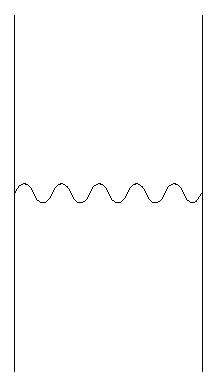
\epsfig{file=witt4a1.eps, width=0.2\linewidth}
\end{center}

Thus we have 
$$
\Gamma_4(p_1,p_2,q_1,q_2)=e^2(G_2((p_1-q_1)^2)+G_2((p_1-q_2)^2)),
$$
where $G_2(p^2)$ is the free photon propagator.
Here $G_2$ is regarded as an operator from $S\o S$ to
$S\o S$, where $S$ is the space of spinors. 

{\bf Remark.} In principle, we should include the diagrams where 
one of the electrons exchanges a photon with itself, 
but we will not consider them, regarding them as absorbed in
the electron propagator. 

To order $e^4$, we have two possiblities. 

1) The electrons could exchange 
two non-interacting photons. The amplitude of the corresponding 
1-loop diagram 

\begin{center}
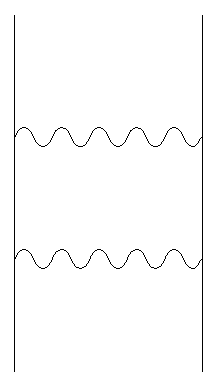
\epsfig{file=witt4a2.eps, width=0.2\linewidth}
\end{center}

can be computed within the framework of QED. 

2) The electrons could exchange only one photon, 
but on its way it could split in an electron and positron, 
 or in a quark and an antiquark. The first splitting scenario

\begin{center}
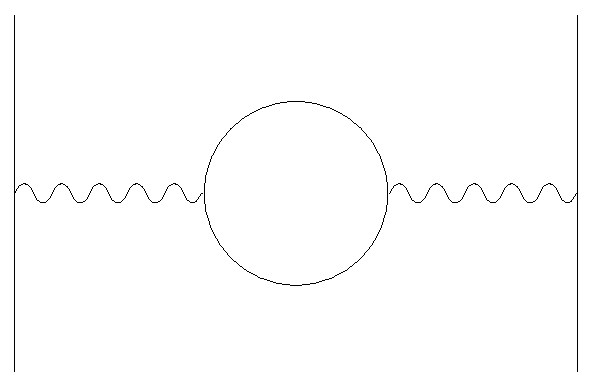
\epsfig{file=witt4a3.eps, width=0.4\linewidth}
\end{center}

is harmless, since it gives only one 1-loop diagram
with no strong interactions, and we can compute the amplitude 
of this diagram as in QED. However, the second scenario (with quarks) 
really gives us trouble. Indeed, the coupling constant
$g$ of the strong interaction is not small, so we 
cannot trust the perturbation expansion in $g$ and thus
have to take into account 
infinitely many Feynman diagrams with any number of loops:

\begin{center}
\epsfig{file=witt4a4.eps, width=0.4\linewidth}
\end{center}

(here dotted lines denote the field of strong 
interaction).
   
However, we know that the theory of strongly interacting quarks
is asymptotically free (when the number of quarks is not too large). 
Thus, we should expect that the perturbative expansion in 
the effective coupling $g_{\text eff}\sim g(\ln p^2)^{-1/2}$ 
should be valid at high momenta. This would mean that at high 
momenta we can restrict to the 1-loop diagrams, which involve no
strong interactions.   
Since we have one such diagram for each type of quark, 

\begin{center}
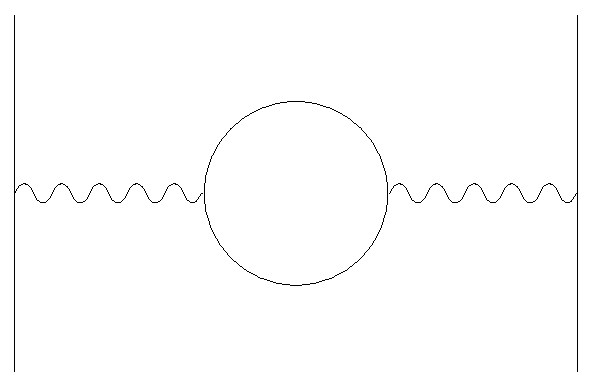
\epsfig{file=witt4a3.eps, width=0.4\linewidth}
\end{center}

the total amplitude
of these diagrams is $\sum e_i^2\Sigma_i(p)$, where
$e_i$ are charges of quarks, and $\Sigma_i$ are amplitudes of 
the corresponding diagrams for a particle with charge 1. 
Of course, the functions $\Sigma_i(p)$ depend on the (unmeasurable!)
masses $m_i$ of quarks, but at high momenta masses are irrelevant,
and all functions $\Sigma_i$ are approximately equal 
to each other. 
Thus, the amplitude is $\Sigma(p)(\sum e_i^2)$, where 
$\Sigma(p)$ is a universal function computed from QED
(as in one of the homework exercises).

It follows from asymptotic freedom that 
the (relative) error of this computation is of order $1/\ln p^2$. 
If we compute the two-loop correction
(still working to order $e^4$),
we will get an additional term of the order $1/\ln p^2$, and
the error will be of order $1/\ln^2p^2$. 
More generally, if we take into account $N$-loop diagrams, 
the error will be of order $1/\ln^Np^2$.
Thus, we get an asymptotic series, with very slowly decaying terms, 
but at very high $p$ one can hope that it gives a reasonably good approximation
to the 4-point scattering amplitude. 
This approximation (to the 0-th order) could in principle be checked 
experimentally, and can be regarded as a confirmation of asymptotic
freedom. 

{\bf Remark.} In practice, asymptotic freedom was checked experimentally
in a different way, but the ideology is similar to the one described
above. 

{\bf Correction to the text of lecture 3} (by Pavel Etingof)

Unfortunately, in Section 3.3 of Lecture 3 there is a
wrong statement (noticed by D.Freed). Namely, the statement 
``$\<...\O(x)\O(x')\>\sim |x-x'|^{-[\O]-[\O']}$'' is incorrect.
 For example, it fails
if $\O'=1$ and $\O$ is a nontrivial operator. 
This statement is
true, however, if $\O'=\O$, which is enough to make the point 
which was being made in the text. 

\end{document}


